\subsection{Módulo de Gestión de Operaciones de Mantenimiento (MTTO)}

\begin{figure}[H]\centering
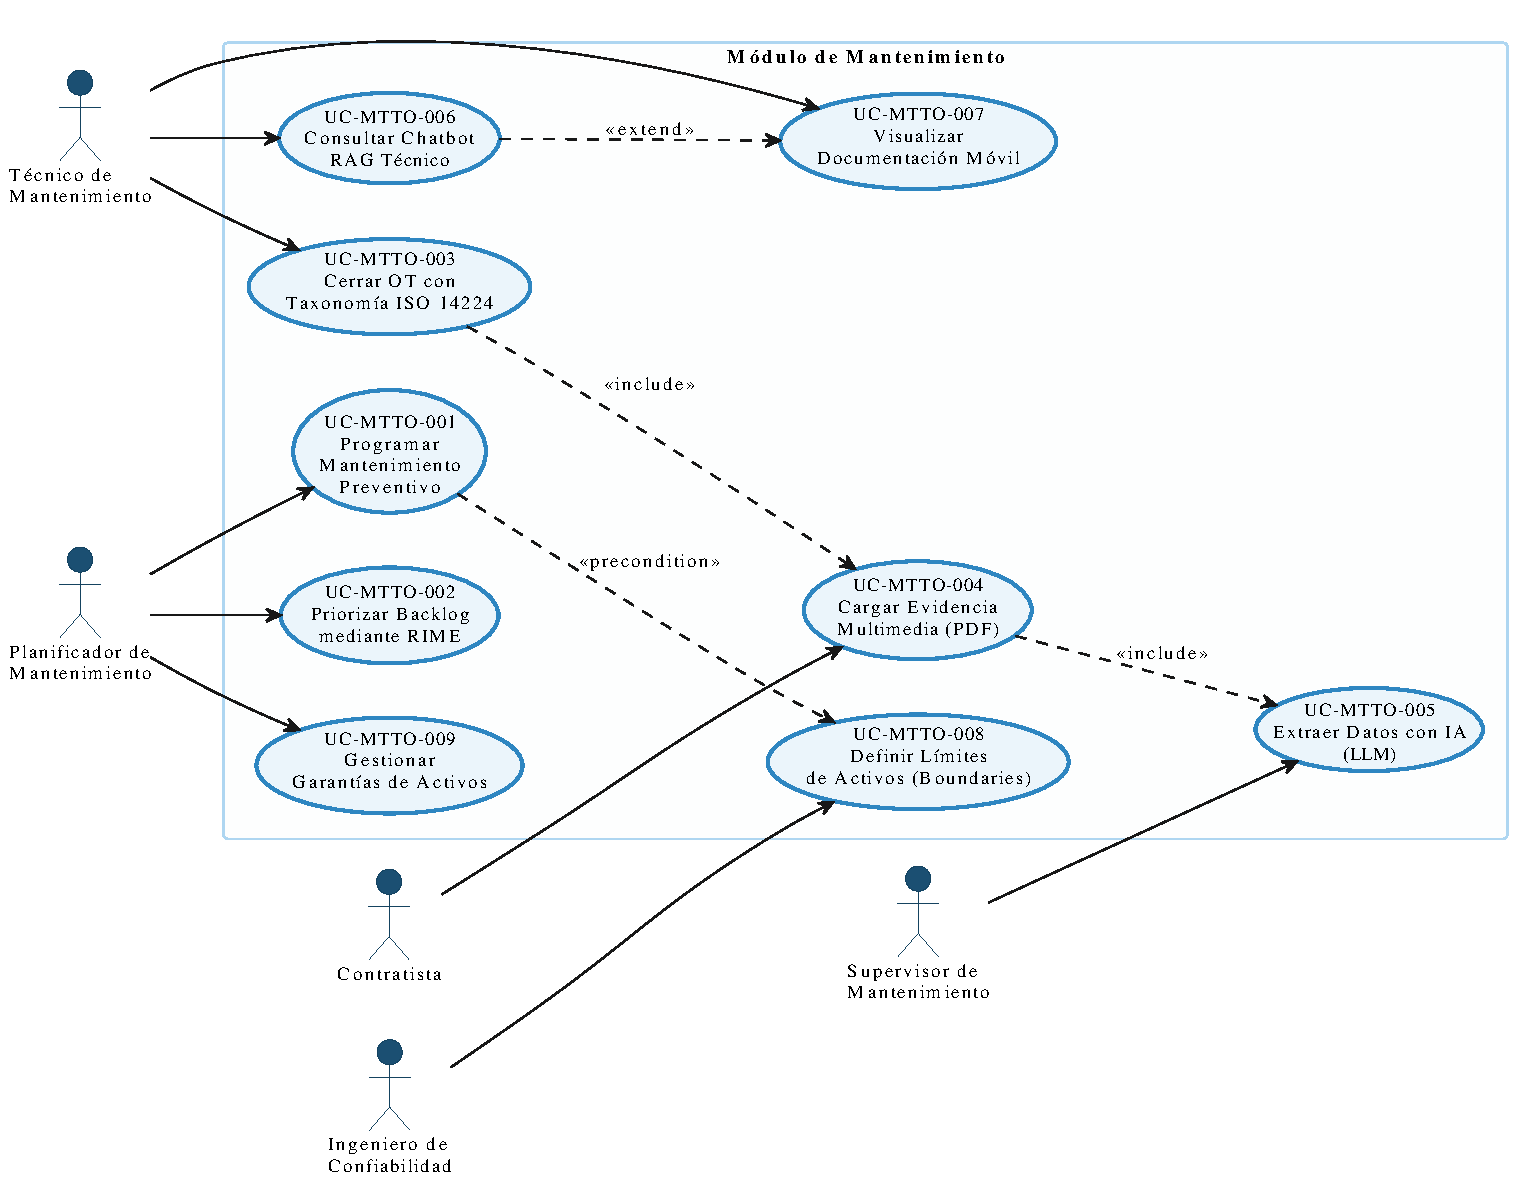
\includegraphics[width=0.85\textwidth]{assets/Diagrama-UC-MTTO.pdf}
\caption{Diagrama de Casos de Uso - Gestión de Operaciones de Mantenimiento}\end{figure}

\noindent\textbf{Ficha de Caso de Uso: UC-MTTO-001 - Programar Mantenimiento Preventivo}
\footnotesize\setlength{\tabcolsep}{4pt}\renewcommand{\arraystretch}{1.2}
\rowcolors{2}{tableBlue}{white}\begin{longtable}{>{\raggedright\arraybackslash}p{0.21\textwidth} >{\raggedright\arraybackslash}p{0.74\textwidth}} \toprule
\textbf{Actor Principal} & Planificador de Mantenimiento \\
\textbf{Actores Secundarios} & Servicio de Planificación de Tareas, Ingeniero de Confiabilidad (notificado) \\
\textbf{Descripción} & Permite crear y programar órdenes de trabajo preventivas recurrentes vinculadas a activos específicos (Nivel 6 ISO 14224) e ítems mantenibles (Nivel 8), con método explícito (time-based o condition-based) y validación de criticidad. \\
\textbf{Precondiciones} & \parbox[t]{\linewidth}{\vspace{2pt} \begin{itemize}[leftmargin=1.5em, nosep, topsep=0pt]
\item El Planificador está autenticado en el sistema con rol ``Planificador de Mantenimiento''
\item El activo está registrado en el catálogo maestro con Tag ISO completo (Nivel 6)
\item El ítem mantenible (Nivel 8) está definido y vinculado al activo
\item Los límites físicos del activo (boundaries) están definidos
\end{itemize} \vspace{2pt}} \\
\textbf{Flujo Principal} & \parbox[t]{\linewidth}{\vspace{2pt} \begin{enumerate}[leftmargin=1.5em, nosep, topsep=0pt]
\item El Planificador accede al módulo de Planificación de Mantenimiento y selecciona ``Crear Plan Preventivo''.
\item El Sistema muestra el formulario de creación con campos obligatorios:
\begin{itemize}[leftmargin=1.2em, nosep, topsep=0pt]
\item Selección de activo (Nivel 6 ISO 14224) mediante búsqueda por Tag.
\item Selección de ítem mantenible (Nivel 8) asociado al activo.
\item Método de mantenimiento (dropdown: ``Time-based'' o ``Condition-based'').
\item Frecuencia (en semanas para time-based, o trigger condition para condition-based).
\item Descripción del trabajo preventivo.
\end{itemize}
\item El Planificador completa todos los campos obligatorios y selecciona método ``Time-based'' con frecuencia ``12 semanas''.
\item El Sistema valida la criticidad del activo:
\begin{itemize}[leftmargin=1.2em, nosep, topsep=0pt]
\item Si criticidad es ``Production Critical'' o ``Safety Critical'' y frecuencia > 8 semanas:
\item Muestra advertencia: ``Para activos Production Critical, se recomienda intervalo $\le$ 8 semanas. ¿Deseas continuar?''
\item El Planificador puede confirmar o modificar el intervalo (FR-003).
\end{itemize}
\item El Planificador confirma la creación del plan.
\item El Sistema:
\begin{itemize}[leftmargin=1.2em, nosep, topsep=0pt]
\item Calcula la próxima fecha de WO basada en la frecuencia configurada (FR-004).
\item Registra en auditoría inmutable [TR-001]: usuario, timestamp, activo Level 6, ítem Level 8, método, frecuencia (FR-006).
\item Crea la primera WO preventiva con estado ``Programada''.
\item Configura el servicio de programación de tareas recurrentes para ejecutar automáticamente.
\end{itemize}
\item El Sistema muestra confirmación: ``Plan creado exitosamente. Próxima WO: [Fecha calculada]''.
\item El Sistema envía notificación al Ingeniero de Confiabilidad con resumen del plan creado.
\end{enumerate} \vspace{2pt}} \\
\textbf{Flujos Alternativos} & \parbox[t]{\linewidth}{\vspace{2pt} \vspace{4pt}\noindent\textbf{AF-001: Campos Obligatorios Incompletos}
\newline
En el paso 3, si el Planificador intenta guardar sin completar campos obligatorios:
\begin{enumerate}[leftmargin=1.5em, nosep, topsep=0pt]
\item El Sistema muestra mensaje de error: ``Campos obligatorios: Activo, Método de Mantenimiento, Frecuencia''.
\item El Sistema resalta los campos faltantes en rojo.
\item El flujo regresa al paso 3.
\end{enumerate}
\vspace{4pt}\noindent\textbf{AF-002: Activo sin Límites Definidos}
\newline
En el paso 4, si el activo no tiene boundaries definidos:
\begin{enumerate}[leftmargin=1.5em, nosep, topsep=0pt]
\item El Sistema muestra mensaje: ``Acción Requerida: El activo seleccionado no tiene límites físicos (Boundaries) configurados. Por favor, contacte al Ingeniero de Confiabilidad para completar la configuración técnica antes de programar el mantenimiento.''
\item El flujo se cancela y regresa a la pantalla principal.
\end{enumerate}
\vspace{4pt}\noindent\textbf{AF-003: Modificación Manual de Intervalo Crítico}
\newline
En el paso 4, si el Planificador modifica el intervalo a $\le$ 8 semanas después de la advertencia:
\begin{enumerate}[leftmargin=1.5em, nosep, topsep=0pt]
\item El Sistema valida el nuevo intervalo.
\item Si es válido, continúa con el paso 5.
\item Registra en auditoría que se modificó el intervalo inicial con justificación ``Ajuste por criticidad''.
\end{enumerate} \vspace{2pt}} \\
\textbf{Postcondiciones} & \parbox[t]{\linewidth}{\vspace{2pt} \begin{itemize}[leftmargin=1.5em, nosep, topsep=0pt]
\item El plan preventivo está activo en el sistema
\item La primera WO está programada con fecha calculada
\item La tarea programada de ejecución recurrente está configurada
\item El historial de auditoría contiene el registro completo de creación
\item El Ingeniero de Confiabilidad ha sido notificado
\end{itemize} \vspace{2pt}} \\
\textbf{Requisitos} & FR-001 a FR-006 [TR-001] \\ \bottomrule
\end{longtable}\normalsize\vspace{1em}
\noindent\textbf{Ficha de Caso de Uso: UC-MTTO-002 - Cerrar OT con Taxonomía ISO 14224}
\footnotesize\setlength{\tabcolsep}{4pt}\renewcommand{\arraystretch}{1.2}
\rowcolors{2}{tableBlue}{white}\begin{longtable}{>{\raggedright\arraybackslash}p{0.21\textwidth} >{\raggedright\arraybackslash}p{0.74\textwidth}} \toprule
\textbf{Actor Principal} & Técnico de Mantenimiento \\
\textbf{Actores Secundarios} & Supervisor de Mantenimiento (revisor), Ingeniero de Confiabilidad (notificado para KPIs) \\
\textbf{Descripción} & Permite al Técnico registrar el cierre de una WO desde un dispositivo móvil, incluyendo Horas Hombre Reales, clasificación de falla según taxonomía ISO 14224 (Ítem Mantenible, Modo, Mecanismo, Causa), y adjuntar evidencia multimedia. Funciona offline con sincronización posterior. \\
\textbf{Precondiciones} & \parbox[t]{\linewidth}{\vspace{2pt} \begin{itemize}[leftmargin=1.5em, nosep, topsep=0pt]
\item El Técnico está autenticado en un dispositivo móvil con rol ``Técnico de Mantenimiento''
\item La WO está asignada al Técnico con estado ``En Progreso''
\item El Técnico ha finalizado físicamente la reparación/mantenimiento
\item El catálogo maestro de taxonomía ISO 14224 está disponible localmente en el dispositivo
\end{itemize} \vspace{2pt}} \\
\textbf{Flujo Principal} & \parbox[t]{\linewidth}{\vspace{2pt} \begin{enumerate}[leftmargin=1.5em, nosep, topsep=0pt]
\item El Técnico abre la WO asignada en su dispositivo móvil y selecciona ``Cerrar Orden de Trabajo''.
\item El Sistema muestra el formulario de cierre con campos obligatorios:
\begin{itemize}[leftmargin=1.2em, nosep, topsep=0pt]
\item Horas Hombre Reales (campo numérico).
\item Ítem Mantenible (dropdown filtrado por clase de activo, Nivel 8 ISO 14224).
\item Modo de Falla (dropdown: ej. ``Fuga Externa'', ``Vibración Excesiva'', ``Sobrecalentamiento'').
\item Mecanismo de Falla (dropdown: ej. ``Erosión'', ``Fatiga'', ``Corrosión'').
\item Causa de Falla (dropdown: ej. ``Desgaste por uso'', ``Error de instalación'', ``Lubricación inadecuada'').
\item Campo opcional: Comentarios adicionales.
\end{itemize}
\item El Técnico ingresa ``8.5'' en Horas Hombre Reales.
\item El Técnico selecciona ``Sello Mecánico'' (Ítem Mantenible Nivel 8).
\item El Sistema filtra los Modos de Falla aplicables a ``Sello Mecánico'' (FR-011 validación jerárquica [TR-008]):
\begin{itemize}[leftmargin=1.2em, nosep, topsep=0pt]
\item Muestra solo: ``Fuga Externa'', ``Desgaste de Cara'', ``Vibración'', etc.
\item Oculta modos irrelevantes como ``Cortocircuito'' o ``Falla de Software''.
\end{itemize}
\item El Técnico selecciona:
\begin{itemize}[leftmargin=1.2em, nosep, topsep=0pt]
\item Modo de Falla: ``Fuga Externa''.
\item Mecanismo de Falla: ``Erosión''.
\item Causa de Falla: ``Desgaste por uso''.
\end{itemize}
\item El Técnico selecciona ``Adjuntar Foto/Video'' y captura una imagen de la reparación finalizada (FR-013).
\item El Sistema:
\begin{itemize}[leftmargin=1.2em, nosep, topsep=0pt]
\item Asocia la imagen a la WO.
\item Verifica la integridad de la evidencia multimedia [TR-003].
\item Si offline: guarda la evidencia de forma segura en el dispositivo hasta sincronizar [TR-007].
\end{itemize}
\item El Técnico presiona ``Finalizar''.
\item El Sistema valida que todos los campos obligatorios están completos (FR-012):
\begin{itemize}[leftmargin=1.2em, nosep, topsep=0pt]
\item Si falta algún campo: muestra error ``Error de cumplimiento ISO 14224: Todos los campos de taxonomía de falla son obligatorios''.
\item Si todos completos: continúa.
\end{itemize}
\item El Sistema:
\begin{itemize}[leftmargin=1.2em, nosep, topsep=0pt]
\item Cambia estado de WO a ``Pendiente de Revisión'' (FR-014).
\item Guarda los datos en el historial del activo con timestamp.
\item Registra en auditoría inmutable [TR-001]: usuario, timestamp, identificador de OT, horas reales, taxonomía completa, evidencia adjunta.
\item Si online: sincroniza inmediatamente con el servidor.
\item Si offline: muestra indicador ``Pendiente de Sincronización'' [TR-007] y registra la operación para sincronización posterior (FR-014).
\end{itemize}
\item El Sistema muestra confirmación: ``WO cerrada exitosamente. Estado: Pendiente de Revisión''.
\item El Sistema envía notificación al Supervisor e Ingeniero de Confiabilidad con resumen de cambios y KPIs actualizados (MTBF/MTTR recalculados).
\end{enumerate} \vspace{2pt}} \\
\textbf{Flujos Alternativos} & \parbox[t]{\linewidth}{\vspace{2pt} \vspace{4pt}\noindent\textbf{AF-001: Campos Obligatorios Incompletos}
\newline
En el paso 10, si faltan campos de taxonomía:
\begin{enumerate}[leftmargin=1.5em, nosep, topsep=0pt]
\item El Sistema muestra error: ``Error de cumplimiento ISO 14224: Faltan campos obligatorios: [Mecanismo de Falla]''.
\item El Sistema resalta el campo faltante en rojo.
\item El flujo regresa al paso 2.
\end{enumerate}
\vspace{4pt}\noindent\textbf{AF-002: Operación Offline}
\newline
En el paso 1, si el Técnico está sin conexión de red:
\begin{enumerate}[leftmargin=1.5em, nosep, topsep=0pt]
\item El Sistema muestra indicador ``Modo Offline'' en la barra superior.
\item Los pasos 1-11 continúan normalmente usando almacenamiento seguro local [TR-007].
\item En el paso 11, el Sistema:
\begin{itemize}[leftmargin=1.2em, nosep, topsep=0pt]
\item Guarda los cambios localmente de forma segura.
\item Marca la operación como pendiente de sincronización automática.
\item Muestra ``WO cerrada localmente. Sincronización pendiente''.
\end{itemize}
\item Cuando conexión se restablece:
\begin{itemize}[leftmargin=1.2em, nosep, topsep=0pt]
\item El Sistema detecta conectividad y procesa las operaciones pendientes (FR-014).
\item Envía datos al servidor con mecanismo de reintento automático en caso de fallos transitorios.
\item Si la sincronización es exitosa: confirma el envío y muestra notificación ``Sincronización completada''.
\end{itemize}
\end{enumerate}
\vspace{4pt}\noindent\textbf{AF-003: Multimedia Dañada o Ilegible}
\newline
En el paso 8, si la imagen capturada está corrupta:
\begin{enumerate}[leftmargin=1.5em, nosep, topsep=0pt]
\item El Sistema detecta que la evidencia no supera la validación de integridad.
\item Muestra error: ``Error al procesar imagen. Por favor captura nuevamente''.
\item Elimina el archivo temporal.
\item El flujo regresa al paso 7.
\end{enumerate}
\vspace{4pt}\noindent\textbf{AF-004: Sincronización Fallida}
\newline
Después del paso 11 (en modo offline):
\begin{enumerate}[leftmargin=1.5em, nosep, topsep=0pt]
\item El Sistema intenta sincronizar con mecanismo de reintento automático.
\item Si los intentos de sincronización agotan la capacidad de reintento:
\begin{itemize}[leftmargin=1.2em, nosep, topsep=0pt]
\item Mantiene la operación en estado de sincronización pendiente con indicador de fallo.
\item Muestra notificación: ``Sincronización falló. Verifique conexión y reintente manualmente''.
\item Registra el evento en el historial de auditoría.
\end{itemize}
\end{enumerate} \vspace{2pt}} \\
\textbf{Postcondiciones} & \parbox[t]{\linewidth}{\vspace{2pt} \begin{itemize}[leftmargin=1.5em, nosep, topsep=0pt]
\item La WO tiene estado ``Pendiente de Revisión''
\item Todos los datos de taxonomía ISO 14224 están registrados en el historial del activo
\item La evidencia multimedia está asociada a la WO con mecanismo de validación de integridad
\item El registro de auditoría inmutable contiene el cierre completo
\item El Supervisor e Ingeniero han sido notificados
\item Los KPIs (MTBF/MTTR) están actualizados en el dashboard
\end{itemize} \vspace{2pt}} \\
\textbf{Requisitos} & FR-010 a FR-014 [TR-001, TR-007, TR-008] \\ \bottomrule
\end{longtable}\normalsize\vspace{1em}
\noindent\textbf{Ficha de Caso de Uso: UC-MTTO-003 - Priorizar Backlog mediante RIME}
\footnotesize\setlength{\tabcolsep}{4pt}\renewcommand{\arraystretch}{1.2}
\rowcolors{2}{tableBlue}{white}\begin{longtable}{>{\raggedright\arraybackslash}p{0.21\textwidth} >{\raggedright\arraybackslash}p{0.74\textwidth}} \toprule
\textbf{Actor Principal} & Planificador de Mantenimiento \\
\textbf{Actores Secundarios} & Ingeniero de Confiabilidad (configurador de pesos), Planificador Avanzado (ajustes manuales) \\
\textbf{Descripción} & Calcula automáticamente la prioridad de Solicitudes de Trabajo (WR) basándose en la matriz RIME (Risk, Impact, Maintainability, Economy), eliminando subjetividad y asegurando que los recursos se enfoquen en problemas de mayor riesgo. \\
\textbf{Precondiciones} & \parbox[t]{\linewidth}{\vspace{2pt} \begin{itemize}[leftmargin=1.5em, nosep, topsep=0pt]
\item El Planificador está autenticado con rol ``Planificador de Mantenimiento''
\item Existen Solicitudes de Trabajo (WR) pendientes de programación
\item Cada activo tiene clasificación de criticidad predefinida (Production Critical, Process Equipment, Support, Non-Critical)
\item Los factores RIME están configurados por el Ingeniero de Confiabilidad (pesos y umbrales)
\end{itemize} \vspace{2pt}} \\
\textbf{Flujo Principal} & \parbox[t]{\linewidth}{\vspace{2pt} \begin{enumerate}[leftmargin=1.5em, nosep, topsep=0pt]
\item El Planificador accede al módulo ``Gestión de Backlog'' y selecciona ``Ver Solicitudes Pendientes''.
\item El Sistema recupera todas las WR con estado ``Nueva'' o ``Pendiente de Programación'' de la base de datos.
\item Para cada WR, el Sistema calcula automáticamente el puntaje RIME (FR-058 a FR-062):
\begin{itemize}[leftmargin=1.2em, nosep, topsep=0pt]
\item Risk (0-25):
\item Criticidad del activo: Production Critical = 25, Proceso = 15, Soporte = 10, No-Crítico = 5.
\item Tipo de fallo: Safety = +10, Environmental = +8, Producción = +5.
\item Impact (0-25):
\item Duración probable de downtime: Crítico (8+h) = 25, Mayor (4-7h) = 18, Moderado (1-3h) = 10, Menor (<1h) = 5.
\item Costo de downtime (configurable por planta).
\item Maintainability (0-25):
\item Facilidad de reparación: Simple = 25, Moderado = 15, Complejo = 8, Muy Complejo = 2.
\item Disponibilidad de repuestos: Disponible = +5, 1-7 días = +2, >7 días = -5.
\item Economy (0-25):
\item Costo estimado: Bajo (<\$1k) = 25, Medio (\$1-5k) = 15, Alto (\$5-20k) = 8, Muy Alto (>\$20k) = 2.
\item RIME Score Final = (Risk + Impact + Maintainability + Economy) / 4 (escala 0-100).
\end{itemize}
\item El Sistema categoriza cada WR en banda RIME (FR-063):
\begin{itemize}[leftmargin=1.2em, nosep, topsep=0pt]
\item Do First (80-100): Código visual crítico.
\item Schedule (60-79): Código visual alto.
\item Plan (40-59): Código visual medio.
\item Wish (0-39): Código visual bajo.
\end{itemize}
\item El Sistema ordena el Tablero de Backlog por RIME Score descendente (highest first) (FR-064).
\item El Sistema muestra la tabla con columnas (FR-065): ID WR \textbackslash\{\}
\end{enumerate} \vspace{2pt}} \\
\textbf{Flujos Alternativos} & \parbox[t]{\linewidth}{\vspace{2pt} \vspace{4pt}\noindent\textbf{AF-001: Ajuste Manual de Factores RIME (Planificador Avanzado)}
\newline
\begin{enumerate}[leftmargin=1.5em, nosep, topsep=0pt]
\item En el paso 9, si el usuario tiene rol ``Planificador Avanzado'':
\begin{itemize}[leftmargin=1.2em, nosep, topsep=0pt]
\item El Planificador Avanzado hace clic en ``Ajustar Factores''.
\item El Sistema muestra formulario editable con los 4 factores (Risk, Impact, Maintainability, Economy).
\item El Planificador Avanzado modifica ``Maintainability'' de 20 a 15 y ingresa justificación: ``Repuestos agotados, tiempo de espera 10 días''.
\item El Sistema:
\item Recalcula RIME Score: (25 + 24 + 15 + 26) / 4 = 22.5 $\rightarrow$ 90.
\item Registra en auditoría [TR-001]: usuario, timestamp, WR\_ID, factor\_modificado (Maintainability), valor\_anterior (20), valor\_nuevo (15), justificación.
\item Actualiza la tabla del backlog con el nuevo RIME Score.
\end{itemize}
\item El Sistema muestra confirmación: ``RIME Score ajustado a 90. Cambio registrado en auditoría''.
\end{enumerate}
\vspace{4pt}\noindent\textbf{AF-002: Falta de Datos para Cálculo}
\newline
\begin{enumerate}[leftmargin=1.5em, nosep, topsep=0pt]
\item En el paso 3, si una WR no tiene criticidad de activo definida:
\begin{itemize}[leftmargin=1.2em, nosep, topsep=0pt]
\item El Sistema asigna valor predeterminado conservador: Risk = 5 (No-Crítico).
\item El Sistema marca la WR con indicador visual ``Datos incompletos para cálculo RIME''.
\item El Sistema sugiere: ``Completar criticidad del activo para cálculo preciso''.
\item La WR se ordena al final del backlog hasta que se complete la información.
\end{itemize}
\end{enumerate}
\vspace{4pt}\noindent\textbf{AF-003: Guardado de Vista Personalizada}
\newline
\begin{enumerate}[leftmargin=1.5em, nosep, topsep=0pt]
\item En el paso 12, si el Planificador aplica filtros múltiples:
\begin{itemize}[leftmargin=1.2em, nosep, topsep=0pt]
\item El Planificador hace clic en ``Guardar Vista Actual''.
\item El Sistema solicita nombre de vista: ``Bomba Crítica
\item Do First``.
\item El Sistema guarda la configuración de filtros en preferencias del usuario.
\item La vista aparece en el menú lateral para acceso rápido futuro.
\end{itemize}
\end{enumerate} \vspace{2pt}} \\
\textbf{Postcondiciones} & \parbox[t]{\linewidth}{\vspace{2pt} \begin{itemize}[leftmargin=1.5em, nosep, topsep=0pt]
\item Todas las WR tienen RIME Score calculado y banda asignada
\item El backlog está ordenado objetivamente por prioridad
\item Los ajustes manuales (si aplica) están registrados en auditoría
\item El Planificador tiene visibilidad clara de las tareas críticas (Do First)
\item Las recomendaciones de consolidación están disponibles para optimizar paradas
\end{itemize} \vspace{2pt}} \\
\textbf{Requisitos} & FR-058 a FR-069 [TR-001] \\ \bottomrule
\end{longtable}\normalsize\vspace{1em}
\noindent\textbf{Ficha de Caso de Uso: UC-MTTO-004 - Consultar Chatbot RAG Técnico}
\footnotesize\setlength{\tabcolsep}{4pt}\renewcommand{\arraystretch}{1.2}
\rowcolors{2}{tableBlue}{white}\begin{longtable}{>{\raggedright\arraybackslash}p{0.21\textwidth} >{\raggedright\arraybackslash}p{0.74\textwidth}} \toprule
\textbf{Actor Principal} & Técnico de Mantenimiento \\
\textbf{Actores Secundarios} & Supervisor de Mantenimiento (revisor de queries), Proveedor de Servicio LLM, Motor de Búsqueda Semántica/Vectorial \\
\textbf{Descripción} & Permite al Técnico hacer preguntas en lenguaje natural al chatbot sobre procedimientos, componentes o manuales técnicos. El sistema busca en documentación técnica y retorna respuestas con referencias explícitas a página/sección del manual, con validación de confiabilidad de las respuestas. \\
\textbf{Precondiciones} & \parbox[t]{\linewidth}{\vspace{2pt} \begin{itemize}[leftmargin=1.5em, nosep, topsep=0pt]
\item El Técnico está autenticado en la aplicación móvil
\item El Técnico tiene conexión de red disponible para consultas
\item Los manuales técnicos están indexados y disponibles en el repositorio de documentación
\item Cada manual está asociado a un activo Level 6 o colección de activos
\item El sistema tiene un servicio de búsqueda semántica y generación de respuestas configurado
\end{itemize} \vspace{2pt}} \\
\textbf{Flujo Principal} & \parbox[t]{\linewidth}{\vspace{2pt} \begin{enumerate}[leftmargin=1.5em, nosep, topsep=0pt]
\item El Técnico está en una WO en campo y necesita consultar un procedimiento técnico.
\item El Técnico abre el panel ``Asistente IA'' desde la WO o menú principal (FR-091).
\item El Sistema muestra interfaz del chatbot con:
\begin{itemize}[leftmargin=1.2em, nosep, topsep=0pt]
\item Historial de chat (preguntas y respuestas previas de la sesión).
\item Campo de entrada de texto ``Escribe tu pregunta...''.
\item Indicador de estado: ``Conectado'' (verde).
\end{itemize}
\item El Técnico ingresa la pregunta en lenguaje natural: ``¿Cuál es la temperatura máxima de operación del rodamiento SKF X-100?''
\item El Sistema:
\begin{itemize}[leftmargin=1.2em, nosep, topsep=0pt]
\item Realiza el procesamiento semántico de la consulta (FR-092).
\item Busca documentos relevantes en el repositorio de conocimiento indexado usando algoritmos de relevancia semántica.
\item Recupera los fragmentos de documentos con un nivel de confianza satisfactorio.
\end{itemize}
\item El Sistema utiliza el servicio de generación de respuestas proporcionando:
\begin{itemize}[leftmargin=1.2em, nosep, topsep=0pt]
\item Contexto del dominio: ``Responde SOLO basándose en la documentación técnica proporcionada. Si no encuentras la información, di que no la tienes.''
\item Pregunta del Técnico.
\item Fragmentos de documentos relevantes encontrados.
\end{itemize}
\item El motor de IA genera respuesta técnica basándose en los fragmentos recuperados (FR-093):
\begin{itemize}[leftmargin=1.2em, nosep, topsep=0pt]
\item ``La temperatura máxima de operación del rodamiento SKF X-100 es 120°C según especificaciones del fabricante.''
\end{itemize}
\item El Sistema agrega cita explícita a la respuesta:
\begin{itemize}[leftmargin=1.2em, nosep, topsep=0pt]
\item ``Fuente: Manual SKF Rodamientos Industriales, página 45, sección 'Especificaciones Técnicas del Modelo X-100'''.
\end{itemize}
\item El Sistema muestra la respuesta en el chatbot con:
\begin{itemize}[leftmargin=1.2em, nosep, topsep=0pt]
\item Respuesta del motor de IA.
\item Cita con formato destacado (negrita).
\item Botón ``Ver Documento Completo'' (FR-098).
\item Indicador de confianza técnica.
\end{itemize}
\item El Sistema registra en auditoría [TR-001] (FR-097):
\begin{itemize}[leftmargin=1.2em, nosep, topsep=0pt]
\item timestamp, usuario\_id, WO\_ID, pregunta (texto completo), respuesta, fuente documentos consultados, nivel de confianza y latencia de respuesta.
\end{itemize}
\item El Técnico hace clic en ``Ver Documento Completo''.
\item El Sistema abre el manual en el visor de documentación del sistema, navegando automáticamente a la sección referenciada.
\item El Técnico confirma la información revisando la documentación completa antes de actuar.
\end{enumerate} \vspace{2pt}} \\
\textbf{Flujos Alternativos} & \parbox[t]{\linewidth}{\vspace{2pt} \vspace{4pt}\noindent\textbf{AF-001: Pregunta Off-Topic}
\newline
\begin{enumerate}[leftmargin=1.5em, nosep, topsep=0pt]
\item En el paso 4, si el Técnico pregunta ``¿Cuál es la capital de Francia?'':
\begin{itemize}[leftmargin=1.2em, nosep, topsep=0pt]
\item El Sistema detecta que la pregunta no está relacionada con documentación técnica.
\item El LLM responde: ``Esa pregunta no está relacionada con mantenimiento. Por favor hazme preguntas sobre equipos o procedimientos técnicos.'' (FR-093).
\item El flujo regresa al paso 3.
\end{itemize}
\end{enumerate}
\vspace{4pt}\noindent\textbf{AF-002: Nivel de Confianza Bajo (Alucinación detectada)}
\newline
\begin{enumerate}[leftmargin=1.5em, nosep, topsep=0pt]
\item En el paso 6, si la respuesta generada tiene un score de confianza técnica bajo (< 70\%):
\begin{itemize}[leftmargin=1.2em, nosep, topsep=0pt]
\item El Sistema no muestra la respuesta directa.
\item El Sistema comunica: ``No puedo darte una respuesta 100\% segura basada solo en los manuales. Aquí están los documentos relevantes para que los verifiques manualmente (FR-093).''
\item Muestra enlaces a las fuentes originales.
\item El flujo continúa en el paso 11.
\end{itemize}
\end{enumerate}
\vspace{4pt}\noindent\textbf{AF-003: Sin Resultados en RAG}
\newline
\begin{enumerate}[leftmargin=1.5em, nosep, topsep=0pt]
\item En el paso 5, si no se encuentran fragmentos relevantes:
\begin{itemize}[leftmargin=1.2em, nosep, topsep=0pt]
\item El Sistema comunica: ``No encontré información sobre eso en la biblioteca técnica actual.''
\item Ofrece opción: ``¿Deseas notificar al Ingeniero de Confiabilidad para que revise este vacío de información?'' (FR-095).
\end{itemize}
\end{enumerate}
\vspace{4pt}\noindent\textbf{AF-004: Timeout del Servicio de Respuesta}
\newline
\begin{enumerate}[leftmargin=1.5em, nosep, topsep=0pt]
\item En el paso 7, si el servicio de generación de respuestas no responde en el tiempo configurado:
\begin{itemize}[leftmargin=1.2em, nosep, topsep=0pt]
\item El Sistema muestra mensaje: ``Tiempo de espera agotado. Por favor intenta nuevamente''.
\item El Sistema registra en auditoría: latencia = timeout, estado = ``error''.
\item El flujo regresa al paso 3.
\end{itemize}
\end{enumerate}
\vspace{4pt}\noindent\textbf{AF-005: Múltiples Preguntas en Sesión}
\newline
\begin{enumerate}[leftmargin=1.5em, nosep, topsep=0pt]
\item Después del paso 13, si el Técnico hace otra pregunta:
\begin{itemize}[leftmargin=1.2em, nosep, topsep=0pt]
\item El Sistema mantiene el contexto de la conversación (historial de chat).
\item Los pasos 4-13 se repiten.
\item Cada pregunta/respuesta se registra independientemente en auditoría.
\item El historial completo de la sesión se asocia a la WO\_ID.
\end{itemize}
\end{enumerate} \vspace{2pt}} \\
\textbf{Postcondiciones} & \parbox[t]{\linewidth}{\vspace{2pt} \begin{itemize}[leftmargin=1.5em, nosep, topsep=0pt]
\item La pregunta y respuesta están registradas en auditoría inmutable
\item El Técnico ha recibido respuesta con referencia explícita al manual
\item El Técnico ha confirmado la información leyendo la fuente original
\item El historial de chat está disponible para revisión del Supervisor
\item El sistema ha incrementado contador de uso de RAG para métricas de adopción
\end{itemize} \vspace{2pt}} \\
\textbf{Requisitos} & FR-091 a FR-098 [TR-001] \\ \bottomrule
\end{longtable}\normalsize\vspace{1em}